\documentclass[aps,prx,twocolumn,longbibliography,nofootinbib,floatfix,superscriptaddress]{revtex4-2}
\usepackage{graphicx}
\usepackage{amsmath,amssymb}
\usepackage{xcolor}
\usepackage[colorlinks=true,linkcolor=blue,citecolor=blue,urlcolor=blue,filecolor=blue]{hyperref}
\usepackage{outlines}
\usepackage{braket}

\graphicspath{{figures/}}

% \newcommand{\ket}[1]{\left|#1\right\rangle}
\newcommand{\TODO}[1]{\textcolor{red}{[TODO: #1]}}

\begin{document}

\title{Low-latency feature extraction for qubit readout}

\author{Cornelis J. van Diepen}
\email[Email to: ]{cjvandiepen@gmail.com}
\affiliation{Quantum Machines, Delft, Netherlands}
\author{Paul Jamet}
\affiliation{Quantum Machines, \textit{elsewhere}}
\author{Tom Dvir}
\affiliation{Quantum Machines, Delft, Netherlands}

\date{\today}

\begin{abstract}
    Pre-measurement state instead of post-measurement state, e.g., due to relaxation during readout. 
\end{abstract}

\maketitle

\section{Introduction}

Figures of merit for readout with QEC
\begin{outline}
    \1 Assignment fidelity
    \1 Readout duration
    \1 Measurement induced transitions
\end{outline}

Flow of the 
Decoder receives error syndrome data as input. 

Relevant concepts related to readout and QEC
\begin{outline}
    \1 Matched filtering: [Phys. Rev. Appl. 7, 054020 (2017, Wallraff group)]
    \1 Soft-decision decoding: 
        \2 first proposal [Pattison, et al. (Microsoft) arXiv:2107.13589], 
        \2 Implemented with superconducting qubits: [Hanisch, APS open science (2026) (Wootton / IBM team)]
    \1 decoder backlog problem: [Skorlic, Terhal]
    \1 decoder switching []
\end{outline}


No reset
\begin{outline}
	\1 \cite{Geher2025}
\end{outline}


\section{Results}

\subsubsection{Pre- and post measurement state}

\begin{figure}[t]
  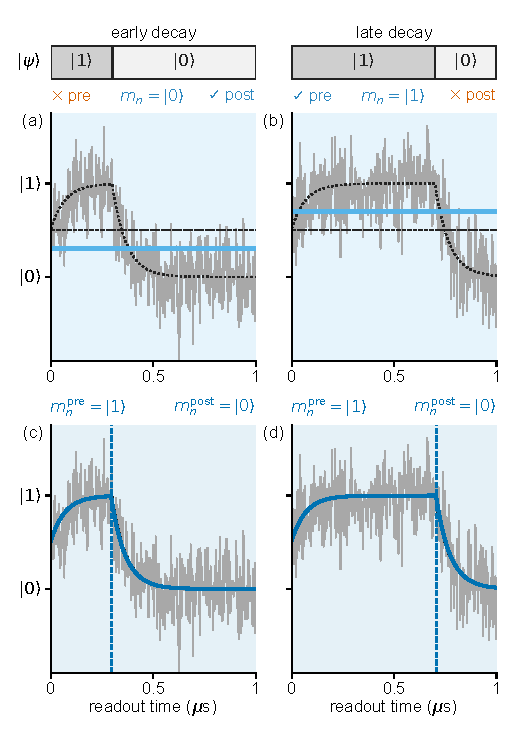
\includegraphics[width=\columnwidth]{fig1_concept.pdf}
  \caption{
  	Effect of qubit relaxation during readout on the assignment of the pre- and post-measurement state. A qubit initially in $\ket{1}$ decays to $\ket{0}$ early (left) or late (right) during the readout; the top row shows the qubit state $\ket{\psi}$ during the readout. 
  	(a),(b)~Conventional assignment: the demodulated signal (grey; dotted: noiseless response) is averaged over the integration window (shaded) and thresholded (dashed line), which gives a single outcome $m_n$ that is used as both the pre- and the post-measurement state.     The pre-measurement state is wrong in~(a) and the post-measurement state is wrong in~(b).
    (c),(d)~Trace-based inference (blue line) detects the decay (dashed line) and returns separate outcomes $m_n^{\mathrm{pre}}$ and $m_n^{\mathrm{post}}$, which are correct in both cases. The traces are synthetic and for illustration only.
    }
  \label{fig:concept}
\end{figure}

Figure~\ref{fig:concept} illustrates how relaxation of the qubit during readout affects the assignment of its state. We consider a qubit prepared in $\ket{1}$ that decays to $\ket{0}$ at a random time while the readout signal is acquired. The top row of Fig.~\ref{fig:concept} shows the qubit state during the readout for an early and a late decay. In the conventional scheme, the demodulated signal is averaged over the readout window and compared to a threshold, so that the entire readout is assigned a single outcome $m_n$. This outcome is subsequently interpreted both as the state before the measurement and as the state after it. For an early decay, the averaged signal falls below the threshold, and the assigned outcome $m_n=\ket{0}$ correctly reflects the post-measurement  state but misidentifies the pre-measurement state, as seen in Fig.~\ref{fig:concept} (a). For a late decay, the averaged signal stays above the threshold, and the assigned outcome $m_n=\ket{1}$ correctly identifies the pre-measurement state but not the post-measurement state, as seen in Fig.~\ref{fig:concept}(b). In both cases a single outcome cannot describe a qubit that changes state during the readout. Analysing the time-resolved readout trace instead makes the decay visible as a change of the signal level at time $t_d$. Figures~\ref{fig:concept}(c) and~\ref{fig:concept}(d) show that this allows the inference of the pre-measurement state $m_n^{\mathrm{pre}}$ and the post-measurement state $m_n^{\mathrm{post}}$ separately. This distinction is essential for experiments in which the post-measurement state of one shot is the initial state of the next. 

\subsubsection{No reset Ramsey}
%Three types of reset protocols: i) thermal reset, ii) active reset, and iii) no reset. 
In a no-reset Ramsey experiment, Fig.~\ref{fig:noreset_ramsey}(a), consecutive shots follow each other without waiting or actively resetting the qubit, so the post-measurement state of readout $n-1$ is the initial state of shot $n$. A shot that starts in $\ket{1}$ gives an inverted fringe, so the outcome of shot $n$ has to be interpreted relative to this initial state,
\begin{equation}
  \tilde m_n = m_n^{\mathrm{pre}} \oplus m_{n-1}^{\mathrm{post}},
  \label{eq:mtilde}
\end{equation}
where $\oplus$ is addition modulo 2. Conventional assignment returns a single outcome $m_n$ and implicitly sets $m_{n-1}^{\mathrm{post}} \equiv m_{n-1}$. This fails when the qubit relaxes during readout: an early $\ket{1}\to\ket{0}$ decay yields a wrong pre-measurement state, and a late decay yields a wrong post-measurement state and hence a mislabelled initial state for the next shot. Relaxation only converts $\ket{1}$ into $\ket{0}$, so outcomes are biased toward $\ket{0}$. Both the oscillation amplitude and the mean of the conventional no-reset fringe are therefore reduced, see Fig.~\ref{fig:noreset_ramsey}(c). Active reset  shown in Fig.~\ref{fig:noreset_ramsey}(b), avoids tracking the initial state, but it adds the feedback latency to every cycle, and a relaxation event during readout leads to a wrong $\pi$ pulse and a residual excitation. Our trace-based inference returns the pre-measurement state $m_n^{\mathrm{pre}}$ and the post-measurement state $m_n^{\mathrm{post}}$ separately, so these errors are removed without any feedback, and the ideal fringe is recovered at the shorter no-reset cycle time.
%
\begin{figure}[htb]
	\centering
	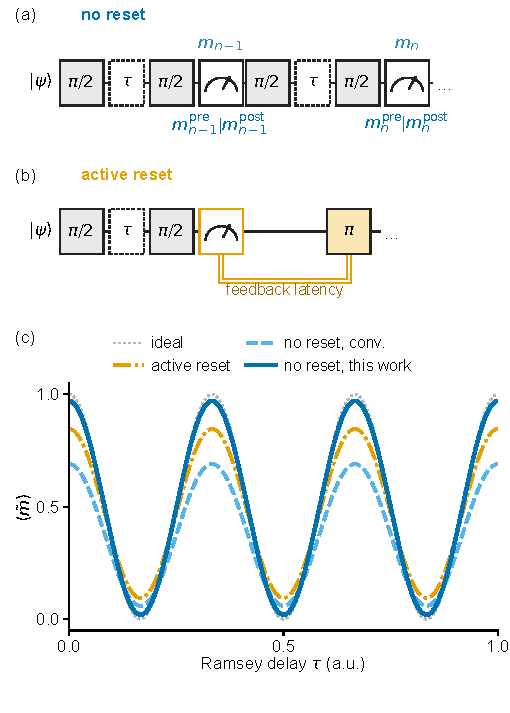
\includegraphics[width=0.9\linewidth]{fig2_sequence.pdf}
	\caption{Ramsey measurement without qubit reset.     
	(a)~In the no-reset protocol, the post-measurement state of readout $n-1$ is the initial state of shot $n$. Conventional assignment (above the meters) gives one outcome $m_n$ used for both states; trace-based inference (below) gives separate pre- and post-measurement states, $m_n^{\mathrm{pre}}$ and $m_n^{\mathrm{post}}$.     
	(b)~Active reset applies a conditional $\pi$ pulse after a feedback latency. 
	(c)~Illustrative Ramsey fringes (schematic, not measured data): relaxation during readout reduces the amplitude and shifts the conventional no-reset curve downward; trace-based inference recovers the ideal fringe without reset.}
		\label{fig:noreset_ramsey}
\end{figure}

\subsubsection{Repetition code}



\section{Conclusion}

\pagebreak
\newpage

\bibliography{refs}

\end{document}